\documentclass{article}
% translate with >> pdflatex -shell-escape <file>

% This file is an extract of the PGFPLOTS manual, copyright by Christian Feuersaenger.
% 
% Feel free to use it as long as you cite the pgfplots manual properly.
%
% See
%   http://pgfplots.sourceforge.net/pgfplots.pdf
% for the complete manual.
%
% Any required input files (for <plot table> or <plot file> or the table package) can be downloaded
% at
% http://www.ctan.org/tex-archive/graphics/pgf/contrib/pgfplots/doc/latex/
% and
% http://www.ctan.org/tex-archive/graphics/pgf/contrib/pgfplots/doc/latex/plotdata/

\usepackage{pgfplots}
\pgfplotsset{compat=newest}

\pagestyle{empty}

\begin{document}
\tikzstyle{every pin}=[fill=white,
	draw=black,
	font=\footnotesize]
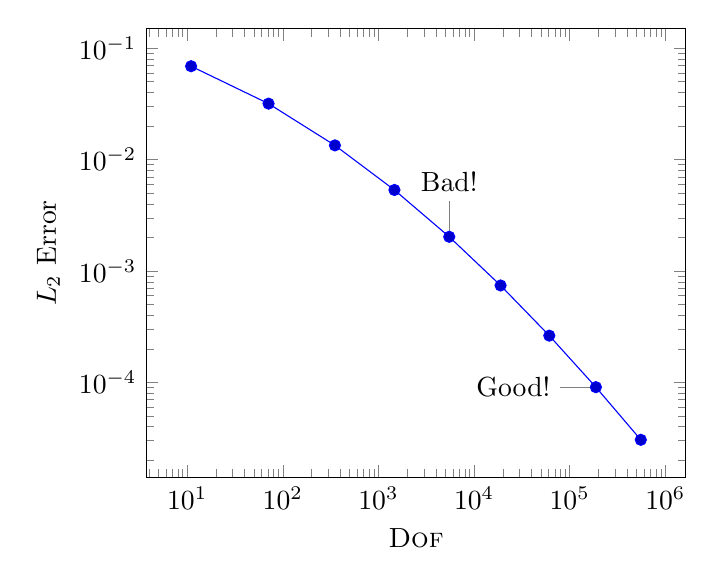
\begin{tikzpicture}
	\begin{loglogaxis}[
		xlabel={\textsc{Dof}},
		ylabel={$L_2$ Error}]

	\addplot coordinates {
		(11,     6.887e-02)
		(71,     3.177e-02)
		(351,    1.341e-02)
		(1471,   5.334e-03)
		(5503,   2.027e-03)
		(18943,  7.415e-04)
		(61183,  2.628e-04)
		(187903, 9.063e-05)
		(553983, 3.053e-05)
	};

	\node[coordinate,pin=above:{Bad!}] 
		at (axis cs:5503,2.027e-03) {};
	\node[coordinate,pin=left:{Good!}] 
		at (axis cs:187903,9.063e-05)	{};
	\end{loglogaxis}
\end{tikzpicture}
\end{document}
